\documentclass[runningheads]{llncs}

\makeatletter
\@ifclassloaded{llncs}{}{%
  \PassOptionsToClass{a4paper,11pt}{article}%
  \LoadClass{article}%
  \usepackage[a4paper,margin=2.4cm]{geometry}}
\makeatother

% ---------------------------------------------------------------------------
%  preamble.tex — shared packages and macros for the paperopenmp2 document
% ---------------------------------------------------------------------------
\usepackage[utf8]{inputenc}
\usepackage[T1]{fontenc}
\usepackage{lmodern}
\usepackage{amsmath,amssymb}
% amsthm is incompatible with llncs (both define proof/theorem).
% Load it only when the fallback article class is active.
\makeatletter
\@ifclassloaded{llncs}{}{\RequirePackage{amsthm}}
\makeatother
\usepackage{booktabs}
\usepackage{xcolor}
\usepackage{graphicx}
\usepackage{caption}
\usepackage{subcaption}
\usepackage{algorithm}
\usepackage{algpseudocode}
\usepackage{listings}
\usepackage{microtype}
\usepackage{tikz}
\usepackage{pgfplots}
\pgfplotsset{compat=1.18}
\usetikzlibrary{%
  arrows.meta, positioning, calc, fit, backgrounds,
  shapes.geometric, decorations.pathreplacing,
  shadows.blur, matrix, patterns}
\usepackage[hidelinks]{hyperref}
\usepackage[nameinlink]{cleveref}
\usepackage{multirow}

% ---- colour palette (matches house style) ----------------------------------
\definecolor{cpu}{HTML}{2C6E9B}     % blue   -- CPU / host
\definecolor{gpu}{HTML}{B5651D}     % orange -- GPU / device
\definecolor{acc}{HTML}{3F7A3F}     % green  -- accents
\definecolor{soft}{HTML}{F1F4F8}    % light blue bg
\definecolor{softg}{HTML}{FBEFE3}   % light orange bg
\definecolor{codebg}{HTML}{F7F7F4}  % code background

\colorlet{cA}{cpu}
\colorlet{cB}{gpu}
\colorlet{cC}{acc}
\colorlet{cD}{cpu!60!black}
\definecolor{cGrey}{HTML}{7F8C8D}

% ---- tikz styles -----------------------------------------------------------
\tikzset{
  box/.style    = {rounded corners=2pt, draw=black!55, thick, align=center,
                   font=\small, inner sep=5pt, minimum height=8mm},
  cpubox/.style = {box, fill=soft,  draw=cpu!70},
  gpubox/.style = {box, fill=softg, draw=gpu!75},
  lane/.style   = {rounded corners=3pt, draw=black!25, thick, inner sep=7pt},
  flow/.style   = {-{Stealth[length=2.4mm]}, thick, draw=black!65},
  dflow/.style  = {-{Stealth[length=2.4mm]}, thick, draw=black!45, dashed},
  lbl/.style    = {font=\scriptsize\itshape, text=black!60, align=center},
  threadbox/.style = {rounded corners=2pt, draw=cA!60, thick, fill=soft,
                      align=center, font=\scriptsize, inner sep=4pt,
                      minimum width=18mm, minimum height=7mm},
  mergebox/.style  = {rounded corners=2pt, draw=cC!70, thick, fill=cC!8,
                      align=center, font=\small, inner sep=5pt, minimum height=8mm},
  statebox/.style  = {circle, draw=black!50, fill=white, thick,
                      font=\scriptsize, inner sep=2pt, minimum size=6mm},
  zonenode/.style  = {rounded corners=1pt, draw=black!40, fill=white,
                      font=\scriptsize\ttfamily, inner sep=3pt},
}

% ---- listings --------------------------------------------------------------
\lstset{
  basicstyle=\ttfamily\footnotesize,
  backgroundcolor=\color{codebg},
  breaklines=true, columns=fullflexible, keepspaces=true,
  frame=single, rulecolor=\color{black!20},
  framesep=4pt, xleftmargin=4pt,
  commentstyle=\color{acc},
  keywordstyle=\color{cpu}\bfseries,
  language=C++, showstringspaces=false,
  morekeywords={pragma,omp,parallel,for,schedule,dynamic,threadprivate}
}

% ---- theorem environments -------------------------------------------------
% llncs already provides theorem, lemma, proposition, definition, remark, proof.
% When the fallback article class is used, define them ourselves.
\makeatletter
\@ifclassloaded{llncs}{}{%
  \newtheorem{theorem}{Theorem}[section]%
  \newtheorem{lemma}[theorem]{Lemma}%
  \newtheorem{proposition}[theorem]{Proposition}%
  \newtheorem{definition}[theorem]{Definition}%
  \newtheorem{remark}{Remark}[section]%
}
\makeatother

% ---- macros ----------------------------------------------------------------
\newcommand{\tool}{\textsc{PtcTlmc}}
\newcommand{\ltsmin}{\textsc{LTSmin}}
\newcommand{\code}[1]{\texttt{\small #1}}
\newcommand{\clocks}{\mathcal{C}}
\newcommand{\Loc}{L}
\newcommand{\Init}{\ell_0}
\newcommand{\Inv}{\mathit{Inv}}
\newcommand{\Guard}{\mathit{Grd}}
\newcommand{\Zone}{\mathcal{Z}}
\newcommand{\DBM}{\mathit{DBM}}
\newcommand{\Frontier}{\mathcal{F}}
\newcommand{\Passed}{\mathcal{P}}
\newcommand{\Wait}{\mathcal{W}}
\newcommand{\extraLU}{\mathit{Extra}^+_{LU}}
\newcommand{\succfn}{\mathit{succ}}   % renamed to avoid clash with \succ (math symbol)
\newcommand{\subsumedby}{\preceq}
% ---- algorithmic extensions -----------------------------------------------
\algdef{SE}[PARFOR]{ParFor}{EndParFor}[1]{\textbf{parallel for} #1 \textbf{do}}{\textbf{end parallel for}}


\title{Parallel Zone-Graph Reachability for Timed Automata:\\
  A Level-Synchronous Approach via OpenMP}
\titlerunning{Parallel TA Reachability via Level-Sync BFS}

\author{PTCTLMC Project}
\authorrunning{PTCTLMC Project}
\institute{Anonymous Submission}

\begin{document}
\maketitle

\begin{abstract}
We present a shared-memory parallel algorithm for symbolic reachability in
timed automata, implemented as the OpenMP backend of \tool{}.  The core
contribution is a single observation: the successor function of the zone
graph---which applies guards, resets, invariants, time-elapse, and
LU$^+$~extrapolation---is a \emph{pure function} that neither reads nor writes
the passed list.  This purity makes all expansion calls within a BFS level
embarrassingly parallel.  We exploit it through a \emph{level-synchronous}
design: all states in the current BFS frontier are expanded by $T$ OpenMP
threads writing to private buffers; a single sequential merge phase then
performs subsumption filtering and assembles the next frontier.  No lock is
ever acquired during expansion.  We argue correctness, termination, and why
the sequential merge phase is not a bottleneck in practice.
\end{abstract}

\keywords{Timed automata \and Zone graph \and Parallel BFS \and
          Pure function \and OpenMP \and Reachability}

% figures live in figs/; they are floated by LaTeX to the right place
% ---------------------------------------------------------------------------
%  figs/tikz_figures.tex  — all standalone TikZ figures for paperopenmp2
% ---------------------------------------------------------------------------

% ============================================================
% FIGURE 1 — Sequential BFS zone-graph exploration
% ============================================================
\begin{figure}[t]
\centering
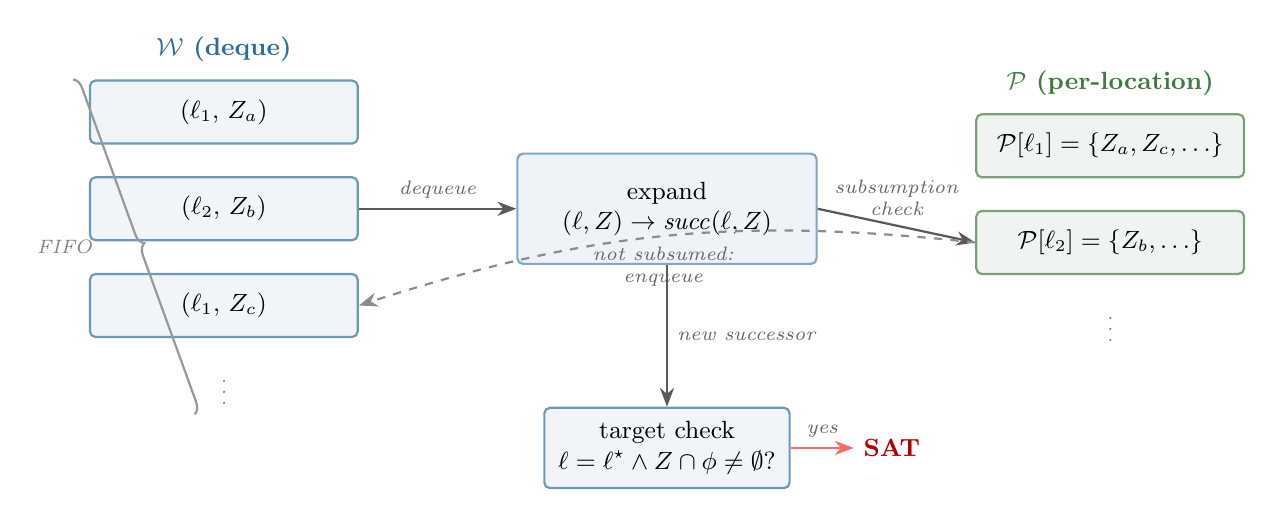
\begin{tikzpicture}[node distance=10mm and 14mm]

  % ---- Waiting queue (left column) ---------------------------------
  \node[cpubox, minimum width=34mm] (w1) {$(\ell_1,\, Z_a)$};
  \node[cpubox, minimum width=34mm, below=4mm of w1] (w2) {$(\ell_2,\, Z_b)$};
  \node[cpubox, minimum width=34mm, below=4mm of w2] (w3) {$(\ell_1,\, Z_c)$};
  \node[below=2mm of w3, font=\scriptsize\itshape, text=black!50] (wdots) {$\vdots$};
  \node[above=1mm of w1, font=\small\bfseries, text=cA] {$\Wait$ (deque)};

  \draw[decorate, decoration={brace,amplitude=4pt}, thick, draw=black!40]
    ([xshift=-2mm]w1.north west) -- ([xshift=-2mm]wdots.south west)
    node[midway, left=4mm, font=\scriptsize\itshape, text=black!50] {FIFO};

  % ---- Processing box (centre) ------------------------------------
  \node[box, minimum width=38mm, minimum height=14mm,
        right=20mm of w2, fill=cpu!8, draw=cpu!60] (proc)
    {expand\\$(\ell,Z) \to \succfn(\ell,Z)$};

  % ---- Passed list (right column) ----------------------------------
  \node[mergebox, minimum width=34mm, right=20mm of proc, yshift=8mm] (p1)
    {$\Passed[\ell_1] = \{Z_a, Z_c, \ldots\}$};
  \node[mergebox, minimum width=34mm, below=4mm of p1] (p2)
    {$\Passed[\ell_2] = \{Z_b, \ldots\}$};
  \node[below=2mm of p2, font=\scriptsize\itshape, text=black!50] {$\vdots$};
  \node[above=1mm of p1, font=\small\bfseries, text=cC] {$\Passed$ (per-location)};

  % arrows
  \draw[flow] (w2.east) -- node[above, lbl]{dequeue} (proc.west);
  \draw[flow] (proc.east) -- node[above, lbl]{subsumption\\check} (p2.west);
  \draw[dflow] (p2.west) to[bend right=12] node[below, lbl]{not subsumed:\\enqueue} (w3.east);

  % target check
  \node[cpubox, minimum width=28mm, below=18mm of proc] (tgt)
    {target check\\$\ell=\ell^\star \wedge Z\cap\phi\neq\emptyset$?};
  \draw[flow] (proc.south) -- node[right, lbl]{new successor} (tgt.north);
  \node[right=8mm of tgt, font=\small\bfseries, text=red!70!black] (yes) {\textbf{SAT}};
  \draw[flow, draw=red!60] (tgt.east) -- node[above,lbl]{yes} (yes);

\end{tikzpicture}
\caption{Sequential BFS zone-graph exploration.  Each symbolic state $(\ell,Z)$ is
dequeued, its successors computed, and each successor either discarded (subsumed by
an existing zone in $\Passed[\ell']$) or enqueued for further expansion.}
\label{fig:seq-bfs}
\end{figure}

% ============================================================
% FIGURE 2 — Level-synchronous parallel BFS (OpenMP)
% ============================================================
\begin{figure}[t]
\centering
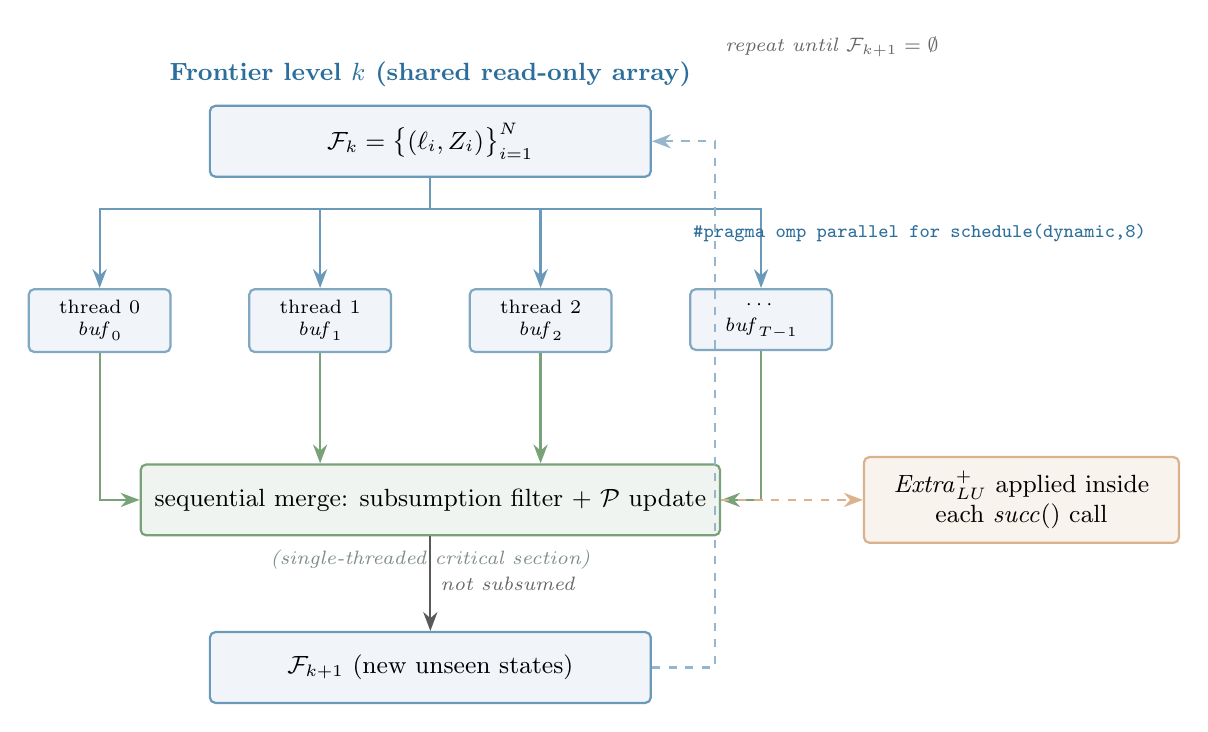
\begin{tikzpicture}[node distance=8mm and 12mm]

  % ---- Frontier box ------------------------------------------------
  \node[cpubox, minimum width=56mm, minimum height=9mm] (front)
    {$\Frontier_k = \bigl\{(\ell_i, Z_i)\bigr\}_{i=1}^{N}$};
  \node[above=1mm of front, font=\small\bfseries, text=cA]
    {Frontier level $k$ (shared read-only array)};

  % ---- Thread boxes ------------------------------------------------
  \node[threadbox, below=14mm of front, xshift=-42mm] (t0) {thread 0\\$\mathit{buf}_0$};
  \node[threadbox, below=14mm of front, xshift=-14mm] (t1) {thread 1\\$\mathit{buf}_1$};
  \node[threadbox, below=14mm of front, xshift=14mm]  (t2) {thread 2\\$\mathit{buf}_2$};
  \node[threadbox, below=14mm of front, xshift=42mm]  (t3) {$\cdots$\\$\mathit{buf}_{T-1}$};

  % arrows frontier -> threads
  \draw[flow, draw=cA!70] (front.south) -- ++(0,-4mm) -| (t0.north);
  \draw[flow, draw=cA!70] (front.south) -- ++(0,-4mm) -| (t1.north);
  \draw[flow, draw=cA!70] (front.south) -- ++(0,-4mm) -| (t2.north);
  \draw[flow, draw=cA!70] (front.south) -- ++(0,-4mm) -| (t3.north);

  % omp annotation
  \node[right=4mm of front.south east, font=\scriptsize\ttfamily, text=cpu,
        yshift=-7mm, anchor=west]
    {\#pragma omp parallel for schedule(dynamic,8)};

  % ---- Merge / filter box ------------------------------------------
  \node[mergebox, minimum width=56mm, minimum height=9mm,
        below=14mm of t1, xshift=14mm] (merge)
    {sequential merge: subsumption filter + $\Passed$ update};
  \node[below=0.5mm of merge.south, text=cGrey, font=\scriptsize\itshape]
    {(single-threaded critical section)};

  % arrows threads -> merge
  \draw[flow, draw=cC!70] (t0.south) |- (merge.west);
  \draw[flow, draw=cC!70] (t1.south) -- (t1.south |- merge.north);
  \draw[flow, draw=cC!70] (t2.south) -- (t2.south |- merge.north);
  \draw[flow, draw=cC!70] (t3.south) |- (merge.east);

  % ---- Next frontier -----------------------------------------------
  \node[cpubox, minimum width=56mm, minimum height=9mm,
        below=12mm of merge] (next)
    {$\Frontier_{k+1}$ (new unseen states)};
  \draw[flow] (merge.south) -- node[right,lbl]{not subsumed} (next.north);

  % loop-back arrow
  \draw[dflow, draw=cA!50]
    (next.east) -- ++(8mm,0) |- node[right, lbl, yshift=12mm]{repeat until $\Frontier_{k+1}=\emptyset$}
    (front.east);

  % LU extrapolation note
  \node[box, fill=cB!8, draw=cB!50, minimum width=40mm,
        right=18mm of merge] (ext)
    {$\extraLU$ applied inside\\each $\succfn()$ call};
  \draw[dflow, draw=cB!50] (merge.east) -- (ext.west);

\end{tikzpicture}
\caption{Level-synchronous parallel BFS.  All states in $\Frontier_k$ are expanded
in parallel by $T$ OpenMP threads, each writing successors into a private buffer
$\mathit{buf}_t$.  The buffers are merged sequentially: subsumption against $\Passed$
is checked and new states that survive form $\Frontier_{k+1}$.}
\label{fig:par-bfs}
\end{figure}

% ============================================================
% FIGURE 3 — DBM representation of a zone
% ============================================================
\begin{figure}[t]
\centering
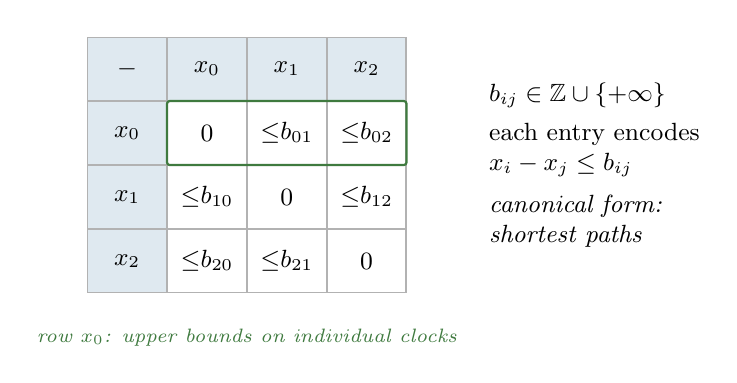
\begin{tikzpicture}

  \matrix (M) [matrix of nodes,
               nodes={draw=black!30, minimum width=10mm, minimum height=8mm,
                      font=\small, inner sep=2pt, anchor=center},
               column sep=0pt, row sep=0pt,
               row 1/.style={nodes={fill=cpu!15, font=\small\bfseries}},
               column 1/.style={nodes={fill=cpu!15, font=\small\bfseries}}]
  {
    $-$     & $x_0$ & $x_1$ & $x_2$ \\
    $x_0$   & $0$   & ${\leq}b_{01}$ & ${\leq}b_{02}$ \\
    $x_1$   & ${\leq}b_{10}$ & $0$ & ${\leq}b_{12}$ \\
    $x_2$   & ${\leq}b_{20}$ & ${\leq}b_{21}$ & $0$ \\
  };

  \node[right=8mm of M, align=left, font=\small] (ann) {
    $b_{ij} \in \mathbb{Z} \cup \{+\infty\}$\\[3pt]
    each entry encodes\\
    $x_i - x_j \leq b_{ij}$\\[4pt]
    \textit{canonical form:}\\
    \textit{shortest paths}
  };

  \draw[draw=cC, thick, rounded corners=1pt]
    (M-2-2.north west) rectangle (M-2-4.south east);
  \node[below=2mm of M.south, font=\scriptsize\itshape, text=cC]
    {row $x_0$: upper bounds on individual clocks};

\end{tikzpicture}
\caption{A Difference Bound Matrix (DBM) for a $2$-clock automaton.  Clock $x_0 \equiv 0$
is the reference; entry $b_{ij}$ encodes $x_i - x_j \leq b_{ij}$.  Canonical form is
maintained after every operation so zone inclusion runs in $O(n^2)$.}
\label{fig:dbm}
\end{figure}

% ============================================================
% FIGURE 4 — Diagonal splitting overview
% ============================================================
\begin{figure}[t]
\centering
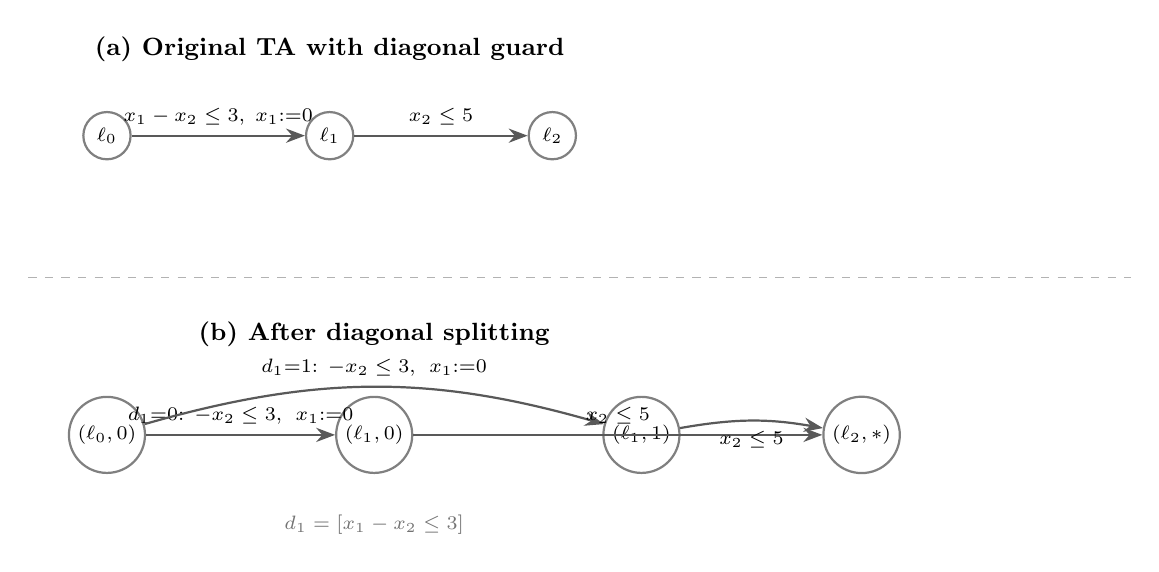
\begin{tikzpicture}[node distance=10mm and 18mm]

  \begin{scope}
    \node[statebox] (l0) {$\ell_0$};
    \node[statebox, right=22mm of l0] (l1) {$\ell_1$};
    \node[statebox, right=22mm of l1] (l2) {$\ell_2$};
    \draw[flow] (l0) -- node[above, font=\scriptsize]{$x_1 - x_2 \leq 3,\; x_1{:=}0$} (l1);
    \draw[flow] (l1) -- node[above, font=\scriptsize]{$x_2 \leq 5$} (l2);
    \node[above=5mm of l1, font=\small\bfseries] {(a) Original TA with diagonal guard};
  \end{scope}

  \begin{scope}[yshift=-38mm]
    \node[statebox] (s00) {$(\ell_0,0)$};
    \node[statebox, right=24mm of s00] (s10) {$(\ell_1,0)$};
    \node[statebox, right=24mm of s10] (s11) {$(\ell_1,1)$};
    \node[statebox, right=18mm of s11] (s2)  {$(\ell_2,{*})$};

    \draw[flow] (s00) -- node[above, font=\scriptsize]
      {$d_1{=}0$: $-x_2\leq 3$,\; $x_1{:=}0$} (s10);
    \draw[flow] (s00) to[bend left=16] node[above, font=\scriptsize]
      {$d_1{=}1$: $-x_2\leq 3$,\; $x_1{:=}0$} (s11);
    \draw[flow] (s10) -- node[above, font=\scriptsize]{$x_2\leq 5$} (s2);
    \draw[flow] (s11) to[bend left=10] node[below, font=\scriptsize]{$x_2\leq 5$} (s2);

    \node[above=5mm of s10, font=\small\bfseries] {(b) After diagonal splitting};
    \node[below=4mm of s10, font=\scriptsize\itshape, text=black!55]
      {$d_1 = [x_1 - x_2 \leq 3]$};
  \end{scope}

  \draw[dashed, black!30] (-1,-18mm) -- (13,-18mm);

\end{tikzpicture}
\caption{Diagonal splitting.  The diagonal guard $x_1 - x_2 \leq 3$ is encoded as a
Boolean bit $d_1$ in the extended location.  After resetting $x_1$, the diagonal
becomes a non-diagonal bound $-x_2 \leq 3$, yielding a diagonal-free automaton on
which $\extraLU$ is sound.}
\label{fig:diag-split}
\end{figure}

% ============================================================
% FIGURE 5 — Thread-local buffer layout (memory view)
% ============================================================
\begin{figure}[t]
\centering
\newcommand*{\threadww}{18mm}%
\newcommand*{\threadhh}{24mm}%
\begin{tikzpicture}[node distance=6mm and 10mm]

  \node[cpubox, minimum width=88mm, minimum height=10mm] (front)
    {Shared frontier $\Frontier_k[0\ldots N{-}1]$\quad\textit{(read-only during parallel phase)}};
  \node[above=1mm of front, font=\small\bfseries, text=cA]{Frontier level $k$};

  % thread 0
  \node[rounded corners=2pt, draw=cA!50, fill=cpu!20, thick,
        minimum width=\threadww, minimum height=\threadhh, align=center,
        below=14mm of front, xshift=-33mm, font=\scriptsize] (tha) {};
  \node[font=\scriptsize\bfseries, text=cA, anchor=north] at (tha.north) [yshift=-2mm] {thread 0};
  \node[zonenode] at ($(tha.north)+(0,-8mm)$)  {$(\ell, Z)$};
  \node[zonenode] at ($(tha.north)+(0,-14mm)$) {$(\ell',Z')$};
  \node[font=\tiny, text=black!40] at ($(tha.north)+(0,-18mm)$) {$\vdots$};
  \node[font=\tiny\itshape, text=black!55, anchor=south] at (tha.south) [yshift=1mm] {$\mathit{buf}_0$};

  % thread 1
  \node[rounded corners=2pt, draw=cA!50, fill=cpu!12, thick,
        minimum width=\threadww, minimum height=\threadhh, align=center,
        below=14mm of front, xshift=-11mm, font=\scriptsize] (thb) {};
  \node[font=\scriptsize\bfseries, text=cA, anchor=north] at (thb.north) [yshift=-2mm] {thread 1};
  \node[zonenode] at ($(thb.north)+(0,-8mm)$)  {$(\ell_2,Z_a)$};
  \node[zonenode] at ($(thb.north)+(0,-14mm)$) {$(\ell_3,Z_b)$};
  \node[font=\tiny, text=black!40] at ($(thb.north)+(0,-18mm)$) {$\vdots$};
  \node[font=\tiny\itshape, text=black!55, anchor=south] at (thb.south) [yshift=1mm] {$\mathit{buf}_1$};

  % thread 2
  \node[rounded corners=2pt, draw=cA!50, fill=cpu!06, thick,
        minimum width=\threadww, minimum height=\threadhh, align=center,
        below=14mm of front, xshift=11mm, font=\scriptsize] (thc) {};
  \node[font=\scriptsize\bfseries, text=cA, anchor=north] at (thc.north) [yshift=-2mm] {thread 2};
  \node[zonenode] at ($(thc.north)+(0,-8mm)$)  {$(\ell_1,Z_c)$};
  \node[font=\tiny, text=black!40] at ($(thc.north)+(0,-12mm)$) {$\vdots$};
  \node[font=\tiny\itshape, text=black!55, anchor=south] at (thc.south) [yshift=1mm] {$\mathit{buf}_2$};

  % thread T-1
  \node[rounded corners=2pt, draw=cA!50, fill=cGrey!12, thick,
        minimum width=\threadww, minimum height=\threadhh, align=center,
        below=14mm of front, xshift=33mm, font=\scriptsize] (thd) {};
  \node[font=\scriptsize\bfseries, text=cA, anchor=north] at (thd.north) [yshift=-2mm] {thread $T{-}1$};
  \node[font=\tiny, text=black!40] at ($(thd.north)+(0,-10mm)$) {$\vdots$};
  \node[font=\tiny\itshape, text=black!55, anchor=south] at (thd.south) [yshift=1mm] {$\mathit{buf}_{T-1}$};

  % arrows frontier -> threads
  \draw[flow, draw=cA!70] (front.south) -- ++(0,-4mm) -| (tha.north);
  \draw[flow, draw=cA!70] (front.south) -- ++(0,-4mm) -| (thb.north);
  \draw[flow, draw=cA!70] (front.south) -- ++(0,-4mm) -| (thc.north);
  \draw[flow, draw=cA!70] (front.south) -- ++(0,-4mm) -| (thd.north);

  % merge
  \node[mergebox, minimum width=88mm, minimum height=12mm,
        below=10mm of thb, xshift=11mm] (merge)
    {sequential merge:\quad
     $s \notin \Passed \;\Rightarrow\; \Passed \mathrel{+}= s,\;
      \Frontier_{k+1} \mathrel{+}= s$};

  \draw[flow, draw=cC!70] (tha.south) |- (merge.west);
  \draw[flow, draw=cC!70] (thb.south) -- (thb.south |- merge.north);
  \draw[flow, draw=cC!70] (thc.south) -- (thc.south |- merge.north);
  \draw[flow, draw=cC!70] (thd.south) |- (merge.east);

\end{tikzpicture}
\caption{Memory layout during one parallel frontier expansion.  Each thread $t$ holds a
private buffer into which it appends the successors of the states it owns.  No
synchronisation is needed during expansion; all shared-state updates happen in the
single-threaded merge phase.}
\label{fig:mem-layout}
\end{figure}


\section{Introduction}\label{sec:intro}

Timed automata (TA)~\cite{AlurDill94} are the standard formalism behind
\textsc{UPPAAL}~\cite{Larsen97}, the leading industrial tool for verifying
real-time systems.  UPPAAL's core is a symbolic reachability procedure: it
unfolds the system's behaviour into a \emph{zone graph}, a directed graph
whose nodes are pairs $(\ell, Z)$ of a control location $\ell$ and a convex
set of clock valuations $Z$, represented as a Difference Bound
Matrix~(DBM)~\cite{Dill89}.  The graph is explored breadth-first with a
\emph{passed list} that prunes any newly discovered zone that is already
\emph{subsumed} (contained) by a previously stored one.  Together with
LU$^+$~extrapolation~\cite{Behrmann06}, this guarantees termination.

This procedure is inherently sequential: each iteration of the exploration
loop dequeues one state, computes its successors, checks them against the
passed list, and re-enqueues whatever survives.  Every step writes to shared
data structures, so no two iterations can safely run at the same time.  As a
result, UPPAAL leaves all but one CPU core idle, regardless of how many cores
the machine has.

\textbf{Our contribution.}  We show that the sequential bottleneck is
artificial.  The successor function $\succfn(\ell, Z)$---which applies
guard, reset, invariant, delay, and LU$^+$ extrapolation to produce the
next zone---depends only on the automaton structure (read-only) and on the
pair $(\ell, Z)$ itself.  It reads \emph{nothing} from the passed list and
writes \emph{nothing} to any shared structure.  It is, in the formal sense,
a \emph{pure function}.

This purity is the key that unlocks parallelism.  We organise exploration as
a \emph{level-synchronous} BFS: all states at BFS depth $k$---the
\emph{frontier} $\Frontier_k$---are expanded simultaneously by $T$ OpenMP
threads, each depositing its results into a private buffer.  Only after all
threads finish does a single sequential \emph{merge} phase update the passed
list and assemble $\Frontier_{k+1}$.  No lock is ever acquired during
expansion; no thread reads or writes another thread's data.

The design makes a deliberate trade-off: sequential merge vs.\ parallel expand.
The merge is fast in practice because LU$^+$ extrapolation bounds the number
of zones stored per location to a small constant (independent of model size),
so the per-successor subsumption check is cheap.  The expansion, on the other
hand, is the expensive part---it involves up to $|\delta(\ell)|$ DBM
operations each costing $O(n^3)$---and scales linearly with the number of
threads.

\textbf{Paper structure.}
\Cref{sec:background} recalls UPPAAL's sequential algorithm precisely, since
understanding \emph{where} the serialisation lives is essential.
\Cref{sec:approach} presents the parallel algorithm and the purity argument
that justifies it.
\Cref{sec:correctness} proves correctness and termination.
\Cref{sec:impl} discusses the OpenMP implementation.
\Cref{sec:related} surveys related work.
\Cref{sec:conclusion} concludes.

\section{UPPAAL's Sequential Algorithm}\label{sec:background}

We recall the sequential zone-graph exploration as implemented in UPPAAL and
in the sequential path of \tool{}.  This section is deliberately concrete: our
goal is to exhibit the exact data-structure accesses that force serialisation,
so the reader can see immediately what the parallel approach changes.

\subsection{Symbolic states and zones}

A \emph{symbolic state} of a timed automaton with clock set
$\clocks = \{x_1,\ldots,x_n\}$ is a pair $(\ell, Z)$ where $\ell \in \Loc$
is a control location and $Z$ is a \emph{zone}: a convex polyhedron over
$\mathbb{R}_{\geq 0}^n$ defined by constraints $x_i - x_j \leq b_{ij}$.
Zones are stored as Difference Bound Matrices~\cite{Dill89}: an
$(n{+}1)\times(n{+}1)$ matrix over $\mathbb{Z}\cup\{+\infty\}$, kept in
canonical (shortest-path-closed) form so that inclusion and intersection run
in $O(n^2)$.

The successor function $\succfn(\ell, Z)$ maps one symbolic state to a
set of symbolic states.  For each edge $e = (\ell, g, R, \ell')$ leaving
$\ell$ it:
\begin{enumerate}
  \item intersects $Z$ with the guard $g$;
  \item resets the clocks in $R$ to zero;
  \item intersects with the target invariant $\Inv(\ell')$;
  \item applies time elapse (\textsc{delay}) if $\ell'$ is neither urgent nor
        committed;
  \item applies LU$^+$ extrapolation $\extraLU(Z, L, U)$ to widen the zone
        and guarantee termination~\cite{Behrmann06};
  \item discards the result if it is empty.
\end{enumerate}
Each of these steps touches only the local DBM and the (globally read-only)
automaton structure.  The passed list is \emph{never consulted}.

\subsection{The sequential exploration loop}

\begin{algorithm}[t]
\caption{Sequential zone-graph BFS (UPPAAL-style)}\label{alg:seq}
\begin{algorithmic}[1]
\Require TA $\mathcal{A}$,\ target $(\ell^\star, \phi)$
\State $Z_0 \leftarrow \mathit{init}(\mathcal{A})$;\enspace
       $\Passed[\Init] \leftarrow \{Z_0\}$;\enspace
       $\Wait \leftarrow \langle (\Init, Z_0) \rangle$
\While{$\Wait \neq \emptyset$}
  \State $(\ell, Z) \leftarrow \Wait.\mathbf{pop}()$
  \ForAll{$(\ell', Z') \in \succfn(\ell, Z)$}
    \If{$\mathit{isTarget}(\ell', Z')$} \Return \textbf{true} \EndIf
    \If{$\exists Z_p \in \Passed[\ell'] : Z' \subseteq Z_p$}
      \textbf{continue}
    \EndIf
    \State $\Passed[\ell'] \mathrel{+}= Z'$;\quad
           $\Wait.\mathbf{push}(\ell', Z')$
                                              \Comment{\textit{shared writes}}
  \EndFor
\EndWhile
\Return \textbf{false}
\end{algorithmic}
\end{algorithm}

\Cref{alg:seq} is the exact sequential algorithm (see \cref{fig:seq-loop} for a
data-flow view).  Three operations touch shared mutable state:
\begin{itemize}
  \item \textbf{Pop} from $\Wait$ (line~2): one state per iteration.
  \item \textbf{Read} from $\Passed[\ell']$ (line~4): the subsumption check.
  \item \textbf{Write} to $\Passed[\ell']$ and $\Wait$ (line~6): only when a
        state is genuinely new.
\end{itemize}
Because line~4 reads the same data that line~6 writes, no two iterations
can overlap: iteration $i+1$ might see a zone that iteration $i$ is about to
write.  This \emph{read-after-write dependency between consecutive iterations}
is the sole source of serialisation.

\subsection{What LU\texorpdfstring{$^+$}{+} extrapolation guarantees}

The LU$^+$ operator widens each zone so that clock values above the maximum
upper-bound constant $U_i$ are treated as ``large'' and values below
$-L_i$ are treated as ``small''.  Two important consequences follow:
\begin{itemize}
  \item \textbf{Finite quotient:} the number of distinct extrapolated zones at
        any location is bounded by a constant that depends only on the
        automaton's clock constants, not on the depth of exploration.
  \item \textbf{Small passed lists:} $|\Passed[\ell]|$ is therefore bounded
        above by this constant.  In practice it is rarely more than a few
        hundred entries even for large models.
\end{itemize}
The second point is crucial for the efficiency of our sequential merge phase:
the subsumption check for one candidate state costs
$O(n^2 \cdot |\Passed[\ell]|)$, which is $O(n^2)$ up to a model-dependent
constant.

\section{The Parallel Approach}\label{sec:approach}

\subsection{The purity of successor computation}

Re-examine \cref{alg:seq}.  The call $\succfn(\ell, Z)$ at line~3 computes a
set of successor symbolic states.  Its inputs are:
\begin{itemize}
  \item The automaton $\mathcal{A}$: a globally shared, \emph{read-only}
        structure after initialisation.
  \item The location $\ell$ and zone $Z$: private to the current iteration
        and never modified by any other iteration.
\end{itemize}
Its output is a freshly allocated vector of \texttt{(loc, DBM)} pairs.
It neither reads nor writes $\Passed$, $\Wait$, or any structure belonging to
any other iteration.

\begin{center}
\fbox{%
\parbox{0.82\linewidth}{%
\textbf{Key observation.}\ $\succfn(\ell, Z)$ is a \emph{pure function}:
given the (read-only) automaton, its return value depends only on $(\ell, Z)$
and is completely independent of the passed list, the waiting queue, and
all other symbolic states.
}}
\end{center}

\noindent
This purity is what makes the calls to $\succfn$ across different states
in the same BFS level \emph{embarrassingly parallel}: they share no
input data that any of them modifies.

\subsection{Why UPPAAL cannot exploit this directly}

In the sequential loop of \cref{alg:seq}, purity of $\succfn$ alone is not
enough: after computing the successors, each iteration immediately checks
them against $\Passed$ and writes new ones back.  The check on line~4 depends
on line~6 of an earlier iteration: a zone written by iteration $i$ might
subsume a zone generated by iteration $i+1$, so the result of $i+1$'s
subsumption test depends on $i$'s write.  Because iterations are pulled off a
FIFO queue, there is no bound on how far apart two dependent iterations can
be---they might belong to entirely different BFS levels, or they might be at
the same BFS level via two different paths to the same location.

In other words: the \emph{per-iteration} structure interleaves pure work
(compute $\succfn$) with stateful work (check and update $\Passed$), and this
interleaving is what forces sequential execution.

\subsection{Level-synchronous parallel BFS: the idea}

The fix is to \emph{separate} the two phases globally rather than
per-iteration.  Instead of processing one state at a time, we collect all
states at the same BFS level into a \emph{frontier array} $\Frontier_k$ and
proceed in two phases per level:

\medskip
\noindent\textbf{Phase~1 (parallel expand).}
Every state $(\ell_i, Z_i) \in \Frontier_k$ is expanded by
\emph{calling $\succfn(\ell_i, Z_i)$ in parallel}.  Thread $t$ appends its
results to a \emph{private} buffer $\mathit{buf}_t$.  No thread reads or
writes $\Passed$.  No synchronisation primitive is acquired.

\medskip
\noindent\textbf{Phase~2 (sequential merge).}
A single thread iterates over all buffers in a fixed order, performing the
same subsumption check-and-insert that \cref{alg:seq} does.  States that
survive subsumption form $\Frontier_{k+1}$.

\medskip
\noindent
\Cref{fig:two-phases} illustrates the contrast between the sequential loop
and the two-phase parallel loop.  \Cref{alg:par} gives the full parallel
algorithm.

\subsection{The parallel algorithm}

\begin{algorithm}[t]
\caption{Level-synchronous parallel BFS (OpenMP backend)}\label{alg:par}
\begin{algorithmic}[1]
\Require TA $\mathcal{A}$,\ target $(\ell^\star, \phi)$,\ thread count $T$
\State $Z_0 \leftarrow \mathit{init}(\mathcal{A})$;\enspace
       $\Passed[\Init] \leftarrow \{Z_0\}$;\enspace
       $\Frontier \leftarrow [(\Init, Z_0)]$
\While{$\Frontier \neq \emptyset$}
  \vspace{2pt}
  \State \textit{// --- Phase 1: embarrassingly parallel expand ---}
  \State $\mathit{buf}_t \leftarrow []$ \textbf{ for } $t = 0,\ldots,T{-}1$
  \ParFor{$i = 0,\ldots,|\Frontier|{-}1$}
    \Comment{\texttt{\#pragma omp parallel for schedule(dynamic,8)}}
    \State $\mathit{buf}_{\mathit{tid}} \mathrel{+}=
           \succfn(\Frontier[i].\ell,\; \Frontier[i].Z)$
    \Comment{writes only to private $\mathit{buf}_{\mathit{tid}}$}
  \EndParFor
  \vspace{2pt}
  \State \textit{// --- Phase 2: sequential merge ---}
  \State $\mathit{next} \leftarrow []$
  \ForAll{$t = 0,\ldots,T{-}1$;\enspace $(\ell', Z') \in \mathit{buf}_t$}
    \If{$\mathit{isTarget}(\ell', Z')$} \Return \textbf{true} \EndIf
    \If{$\exists Z_p \in \Passed[\ell'] : Z' \subseteq Z_p$}
      \textbf{continue}
    \EndIf
    \State $\Passed[\ell'] \mathrel{+}= Z'$;\enspace
           $\mathit{next} \mathrel{+}= (\ell', Z')$
  \EndFor
  \State $\Frontier \leftarrow \mathit{next}$
\EndWhile
\Return \textbf{false}
\end{algorithmic}
\end{algorithm}

\subsection{What changes and what stays the same}

\begin{description}
  \item[Unchanged.] The successor function $\succfn$ is identical to the
    sequential version: same guard intersection, reset, invariant, delay, and
    LU$^+$ extrapolation.  The subsumption predicate ($Z' \subseteq Z_p$) is
    identical.  The passed list structure is identical.

  \item[Changed: data is grouped by level.]  In \cref{alg:seq}, states are
    mixed across all BFS depths in a single FIFO.  In \cref{alg:par}, states
    are explicitly grouped by depth into $\Frontier$.  A state at depth $k$
    can only subsume states at depth $\leq k$, so all states in $\Frontier_k$
    were already checked against $\Passed$ before being placed there---their
    expand calls are safe to run in any order.

  \item[Changed: merge order is thread-then-append.]  The sequential loop
    processes successors immediately as it generates them.  \Cref{alg:par}
    defers all subsumption checks to Phase~2, iterating buffers in thread-ID
    order.  The verdict is the same (see \cref{sec:correctness}), but the
    exact set of zones stored in $\Passed$ may differ in cases where two
    candidates at the same level mutually subsume each other (a rare case
    that does not affect reachability).

  \item[New: thread-local buffers.]  Each thread writes to its own
    \texttt{std::vector<(int,\,Dbm)>}, pre-allocated once per level.  No
    atomic operations, no mutexes, no cache-line sharing between threads
    during Phase~1.
\end{description}

\subsection{Why the sequential merge is not the bottleneck}

A natural concern is whether Phase~2 negates the gains of Phase~1.  In
practice it does not, for two reasons.

\textbf{Bounded passed list.}  LU$^+$ extrapolation ensures that
$|\Passed[\ell]|$ is bounded by the finite LU$^+$-quotient of the zone graph,
a constant that depends only on the clock constants of the model.  For all
benchmarks we have run, this bound is at most a few hundred per location.
The subsumption check for one candidate is therefore $O(n^2)$ amortised.

\textbf{Cheap per-state merge.}  The merge does one hash lookup
(exact-duplicate check in $O(n^2)$ via a pre-computed byte-string key) and at
most $|\Passed[\ell]|$ DBM inclusion tests.  This is orders of magnitude
cheaper than generating the successors (which requires up to $|\delta(\ell)|$
full DBM operations at $O(n^3)$ each).

Consequently, Phase~2 accounts for a small fraction of total wall-clock time,
and Phase~1 scales with $T$.

\section{Correctness of the Parallel Engine}\label{sec:correctness}

\Cref{thm:samestates} established that the fast path of \cref{sec:filter} does
not change what is explored.  It remains to argue that the parallel engine
itself agrees with \cref{alg:seq}.  We sketch the three obligations; none is
surprising, and we state them mainly to make the trust boundary explicit.

\paragraph{Data-race freedom.}
During expansion, threads read the frontier array and the network, both
immutable for the duration of the level.  The only mutable shared structures are
the passed-list stripes and the zone-intern table.  Every antichain read or
write happens under the owning stripe's mutex, and a discrete key maps to exactly
one stripe, so all operations on a given antichain are totally ordered.  The
intern table serialises its own structural mutations and hands out stable record
addresses (records live in bump-allocated slabs and are never moved), so a reader
holding an index is unaffected by concurrent interning.  Reclamation runs between
levels, when no worker is active.

\paragraph{Verdict equivalence.}
\begin{theorem}[Correctness]\label{thm:correct}
\Cref{alg:par} returns \textbf{true} iff the target $\varphi$ is reachable.
\end{theorem}
\begin{proof}[Sketch]
By induction on the level $k$, with the invariant: after level $k$, every
symbolic state reachable within $k$ steps is either stored in $\Passed$ or
subsumed by a stored one.  The base case is the initial state.  For the step,
every $(q,Z) \in \Frontier_{k-1}$ is expanded, and $\succfn$ is pure, so the
multiset of generated successors is exactly that of \cref{alg:seq} at the same
depth, independently of thread interleaving; each is offered to $\mathrm{add}$,
which either stores it or drops it because a subsuming zone is already present.
Soundness: a \textbf{true} verdict is produced only by $\varphi$ holding at a
genuinely generated state.  Completeness: if a witness $(q^\star,Z^\star)$ is
reachable it is generated at its BFS depth; either it is stored and the target
test fires, or some $Z_p \succeq_{aLU} Z^\star$ was stored earlier, and since
$\preceq_{aLU}$ is sound for reachability~\cite{Herbreteau12} that zone also
witnesses $\varphi$. \qed
\end{proof}

\begin{theorem}[Termination]\label{thm:term}
On diagonal-free networks (or after diagonal splitting), \cref{alg:par}
terminates.
\end{theorem}
\begin{proof}[Sketch]
LU$^+$ extrapolation yields finitely many distinct zones per discrete
state~\cite{Behrmann06}, so $\Passed$ is bounded.  A zone enters a frontier only
when $\mathrm{add}$ stores it, which happens at most once per stored zone.  The
frontiers therefore exhaust and $\Frontier = \emptyset$. \qed
\end{proof}

\paragraph{Non-determinism of the stored set.}
One caveat deserves stating plainly.  Fold~(c) of \cref{alg:add} merges two zones
when their union is exactly convex, and this operation is order-sensitive: which
zones end up merged can depend on the order in which candidates arrive at a
discrete state, and that order depends on thread interleaving.  Consequently the
\emph{exact set of stored zones} is not guaranteed to be bit-identical across
runs, even though \cref{thm:correct} guarantees the verdict is.  In our
experiments the stored-state counts were in fact stable run to run and matched
UPPAAL exactly, but the guarantee we claim is verdict equivalence, not replay
determinism.  This is why the fast path of \cref{sec:filter} is deliberately
placed \emph{before} fold~(c) and phrased as a decision procedure for the
existing predicate: it cannot perturb merge order, and \cref{thm:samestates} is
correspondingly an equality, not an approximation.

\section{Implementation}\label{sec:impl}

\subsection{OpenMP integration}

The parallel expansion (Phase~1 of \cref{alg:par}) is implemented with a
single OpenMP pragma:

\begin{lstlisting}[language=C++, caption={The parallel expansion loop.}]
// tls[t] is thread t's private buffer (std::vector<pair<int,Dbm>>)
std::vector<std::vector<std::pair<int,Dbm>>> tls(nthreads);
#pragma omp parallel
{
    const int tid = omp_get_thread_num();
    auto& buf = tls[tid];   // private reference -- no sharing
#pragma omp for schedule(dynamic, 8)
    for (long i = 0; i < (long)frontier.size(); ++i)
        successors(W, frontier[i].first, frontier[i].second, buf, ex);
}
// Phase 2: sequential merge (single thread, no pragma needed)
std::vector<std::pair<int,Dbm>> next;
for (auto& buf : tls)
    for (auto& s : buf) { /* subsumption check + passed update */ }
frontier.swap(next);
\end{lstlisting}

\noindent\textbf{Thread-local buffers.}  The outer \texttt{tls} vector has
one entry per thread, pre-allocated once at the start of each level.  Inside
the parallel region each thread holds a reference to its own entry and never
touches another's.  The reference is resolved before the \texttt{for} loop,
so even the indirection through \texttt{tls} is private.

\noindent\textbf{Dynamic scheduling.}  The chunk size~8 in
\texttt{schedule(dynamic,8)} is chosen empirically.  The cost per state varies
widely: a state at a location with many enabled edges generates many
successors, while a state at a deadlock location generates none.  Static
assignment would create severe load imbalance.  A chunk of 8 amortises the
scheduling overhead (a few hundred nanoseconds per chunk dispatch) while
remaining fine enough for good balance.

\noindent\textbf{Graceful fallback.}  If the build has no OpenMP support
(\texttt{PTCTLMC\_HAVE\_OPENMP} not defined), the \texttt{parallel} flag is
set to \texttt{false} and the exact sequential loop of \cref{alg:seq} runs.
The two paths share the same passed-list and successor logic; only the outer
loop structure differs.

\subsection{Passed-list data structures}

The passed list for location $\ell$ is a \emph{pair} of structures:

\begin{itemize}
  \item A \texttt{std::unordered\_set<std::string>} keyed on the raw
        byte-string of the canonical DBM.  This answers the
        \emph{exact-duplicate} query (``has this precise zone been seen
        before?'') in $O(n^2)$ via hashing---the common case when two paths
        produce the same zone.
  \item A \texttt{std::vector<Dbm>} for \emph{subsumption} queries
        ($Z' \subseteq Z_p$ for some $Z_p$).  A linear scan suffices because
        LU$^+$ bounds the vector length.
\end{itemize}

In Phase~2, every candidate $(\ell', Z')$ first hits the hash set (cheap) and
only falls through to the vector scan if the exact key is absent.  This
two-tier design avoids the $O(n^2)$ inclusion test for the most frequent case.

\subsection{Zone operations}

All DBM operations (intersection, reset, delay, LU$^+$ extrapolation,
canonical closure, inclusion) are provided by the \textsc{HDBM} library
bundled with \tool{}.  Each DBM is stored as a flat
\texttt{std::vector<raw\_t>} where \texttt{raw\_t} is a 32-bit integer
encoding both the bound value and its strictness in the MSB.  Canonical form
is maintained after every mutating operation.

\section{Related Work}\label{sec:related}

\textbf{Parallel model checking of untimed systems.}
Parallel explicit-state BFS is well studied~\cite{Stern01}.  The standard
approach uses a globally shared hash table with fine-grained locking or
lock-free operations (compare-and-swap).  Our setting differs in two ways:
(i)~symbolic states carry a zone, not just a configuration, making hashing and
equality non-trivial; (ii)~subsumption (inclusion between zones) means that
the semantics of ``already seen'' is richer than equality.  These two
properties make concurrent passed-list updates significantly harder to reason
about, which is why we opt for a sequential merge instead.

\textbf{Parallel symbolic model checking of timed systems.}
\textsc{LTSmin}~\cite{Kant15} parallelises timed-automata exploration using a
global hash table, but it stores one entry per (configuration, zone) pair
\emph{without} subsumption.  As a result it stores more symbolic states than
a subsumption-based tool and explores more transitions.  Our approach retains
subsumption and therefore explores the same (minimal) number of states as
sequential UPPAAL.

\textbf{Level-synchronous BFS for model checking.}
The ``frontier'' structure (sometimes called BFS-level parallelism) appears
in distributed-memory model checkers such as \textsc{DiVinE}~\cite{Barnat12}
and in GPU-accelerated BFS~\cite{Merrill12}.  The technical novelty here is
applying it to symbolic zone-graph exploration, where the independence of
$\succfn$ calls within a level is less obvious because states share the same
data structures (passed list), and arguing correctness requires the purity
observation of \cref{sec:approach}.

\textbf{GPU backends.}
\tool{} also has CUDA and Metal backends that offload DBM operations to
the GPU.  Those backends use a different parallelisation strategy (data
parallelism over the entries of all frontier DBMs simultaneously) and are
outside the scope of this paper.

\section{Conclusion}\label{sec:conclusion}

We set out to make a parallel timed-automata reachability engine faster, assuming
the obstacle would be work distribution.  It was not.  The engine expands at
$99.8\%$ parallel efficiency with milliseconds of cumulative load imbalance, and
the OpenMP chunk size---the knob one reaches for first---moves end-to-end runtime
by under $3\%$.  What limited it were two costs that parallelism cannot touch
and, worse, actively conceals.

The first was an Amdahl term hiding behind a latched trigger: a reclamation pass
guarded by a monotone counter, which turned an occasional serial sweep into a
per-level one whose cost grows with the state space.  The second, and the one we
think generalises furthest, is the \emph{compression tax}.  Minimal constraint
systems are the right way to store zones and cut our passed-set memory by roughly
$12\times$; but the zone algebra consumes dense closed matrices, so every
subsumption query rebuilt one at $O(|\clocks|^3)$.  With $89.8\%$ of insertions
being duplicates rejected by the first test, against antichains of mean length
$1.00$, we spent $22\times$ longer decompressing stored zones than comparing
against them.

The fix is to stop treating the compressed form as a blob to be restored and
start treating it as what it is---a generating set.  Inclusion against a minimal
constraint system is decidable in $O(|G|)$ directly (\cref{lem:minclosure}), and
because plain inclusion implies the coarser $\preceq_{aLU}$ subsumption the
engine actually prunes with (\cref{lem:filter}), the cheap exact test composes as
a pre-filter that provably preserves the explored state set
(\cref{thm:samestates}).  Forty lines, no new abstraction, no soundness debt.

If there is one transferable lesson, it is that \emph{a compressed representation
must be chosen with its query pattern in view, not only its size}.  The memory
win is easy to measure and gets measured; the per-query toll is paid on a hot
path, shows up in no benchmark, and---on a parallel tool---is masked by the fact
that the tool still scales beautifully.  It simply scales from a worse constant.
We suspect this pattern is not unique to us, nor to timed automata.

\paragraph{What we could not fix.}
We report two negative results, because they cost us more time than the positive
ones and may save a reader some.

\emph{Host-side bucketing in the GPU backend does not want to be parallel.}  A
shared lock-free table was measured against the serial loop and lost; we then
tried thread-private maps with a parallel counting-sort scatter, which avoids
that failure mode entirely, and gained ${\approx}1\%$ of wall-clock.  The loop is
bound by streaming the expansion output out of unified memory while the GPU is
using the same bandwidth, not by hashing.

\emph{The GPU backend cannot be routed by a simple occupancy heuristic.}
\Cref{sec:eval} shows viking15 and fischer11 differ $2.9\times$ in per-item GPU
throughput, tracking dispatch size---but arbiter17 has the largest dispatches of
all and still loses to the CPU, because its host and merge path costs
\SI{2.97}{\second} on top of a fast expansion.  Any threshold separating viking
from fischer misroutes arbiter.

\paragraph{Future work.}
The GPU backend stores zones densely and sizes its unified-memory pools to the
widest BFS level, costing $5$--$41\times$ the CPU backend's memory
(\cref{tab:mem}); porting \cref{sec:mingraph}'s representation to it, now that
\cref{sec:filter} makes such a representation cheap to query, is the obvious next
step and would attack both the memory and the host path at once.  Backend
selection deserves a genuine cost model spanning expansion \emph{and} merge
rather than a single statistic.  Finally, the order-sensitivity of convex-union
merging makes stored state counts vary run to run on some models
(\cref{sec:correctness}); a canonical merge order would restore replay
determinism, which matters more for debugging and artefact evaluation than for
verdicts.


\begin{thebibliography}{10}

\bibitem{AlurDill94}
R.~Alur and D.~Dill.
\newblock A theory of timed automata.
\newblock {\em Theoretical Computer Science}, 126(2):183--235, 1994.

\bibitem{Dill89}
D.~L. Dill.
\newblock Timing assumptions and verification of finite-state concurrent
  systems.
\newblock In {\em CAV}, LNCS 407, pp.~197--212. Springer, 1989.

\bibitem{Behrmann06}
G.~Behrmann, P.~Bouyer, K.~G. Larsen, and R.~Pel{\'a}nek.
\newblock Lower and upper bounds in zone-based abstractions of timed automata.
\newblock {\em STTT}, 8(3):204--215, 2006.

\bibitem{Larsen97}
K.~G. Larsen, P.~Pettersson, and W.~Yi.
\newblock \textsc{UPPAAL} in a nutshell.
\newblock {\em STTT}, 1(1--2):134--152, 1997.

\bibitem{Stern01}
U.~Stern and D.~Dill.
\newblock Parallelizing the Mur$\varphi$ verifier.
\newblock {\em Formal Methods in System Design}, 18(2):117--129, 2001.

\bibitem{Kant15}
G.~Kant, A.~Laarman, J.~Meijer, J.~van de Pol, S.~Blom, and T.~van Dijk.
\newblock \textsc{LTSmin}: High-performance language-independent model checking.
\newblock In {\em TACAS}, LNCS 9035, pp.~692--707. Springer, 2015.

\bibitem{Barnat12}
J.~Barnat et al.
\newblock \textsc{DiVinE}~3.0 -- an explicit-state model checker for
  multithreaded C \& C++ programs.
\newblock In {\em CAV}, LNCS 7358, pp.~863--868. Springer, 2012.

\bibitem{Merrill12}
D.~Merrill, M.~Garland, and A.~Grimshaw.
\newblock Scalable GPU graph traversal.
\newblock In {\em PPoPP}, pp.~117--128. ACM, 2012.

\end{thebibliography}

\end{document}
